\chapter{Simulation Results}
\label{ch:simulation-results}

\epigraph{In God we trust; all others must bring data.}{--- W. Edwards Deming}

\lettrine[lines=2]{T}{he simulations reveal} a striking 22-fold difference in untreated tumor burden between male and female virtual patients, and demonstrate that combination ICI+TKI therapy achieves 65\% survival in female cohorts---a prediction consistent with emerging sex-stratified clinical evidence. This chapter presents results from systematic simulation across eight scenarios: sex-specific baseline conditions and three treatment modalities (ICI, TKI, combination) stratified by biological sex. Single-seed results first illustrate representative dynamics, followed by a 160-simulation multi-seed study that characterizes stochastic variability and provides statistically grounded efficacy estimates.

% ======================================================================
\section{Baseline Simulation}
\label{sec:baseline-sim}

Male patients exhibited aggressive tumor progression, reaching 2,034 tumor cells over 287 steps with 29 immune-mediated kills and mean glucose of 5.042. This rapid expansion was driven by higher initial mutational burden (3 BRCA1 mutations versus 1 in females), testosterone-mediated suppression of CD8$^+$ T~cells, and extensive tumor-driven angiogenesis sustaining glucose supply. Female patients followed a markedly different trajectory: only 92 final tumor cells over 299 steps, 15 kills, and mean glucose of 3.167---a 22-fold reduction reflecting both the lower mutation count and estrogen-enhanced Th1-type immune responses.

% ======================================================================
\FloatBarrier
\section{Treatment Scenarios}
\label{sec:treatment-scenarios}

Three treatment modalities were evaluated across both sexes, activating after step 100 to allow baseline disease establishment. Table~\ref{tab:treatment-outcomes} summarizes the complete single-seed results.

\begin{table}[htbp]
\centering
\caption{Simulation outcomes across all treatment scenarios and biological sex.}
\label{tab:treatment-outcomes}
\begin{tabular}{lllrrrl}
\toprule
\textbf{Scenario} & \textbf{Outcome} & \textbf{Final Tumor} & \textbf{Steps} & \textbf{Kills} & \textbf{Mean Glucose} \\
\midrule
Male, No Tx & PROGRESSION & 2034 & 287 & 29 & 5.042 \\
Female, No Tx & PROGRESSION & 92 & 299 & 15 & 3.167 \\
Male, TKI & SURVIVAL & 0 & 222 & 11 & 2.606 \\
Female, TKI & SURVIVAL & 0 & 113 & 11 & 2.370 \\
Male, ICI & SURVIVAL & 0 & 143 & 11 & 2.370 \\
Female, ICI & SURVIVAL & 0 & 129 & 11 & 2.480 \\
Male, ICI+TKI & SURVIVAL & 0 & 162 & 11 & 2.562 \\
Female, ICI+TKI & PROGRESSION & 6 & 299 & 10 & 2.984 \\
\bottomrule
\end{tabular}
\end{table}

All three regimens achieved tumor elimination in males: ICI fastest (143 steps), then ICI+TKI (162), then TKI (222).  Females cleared tumors faster under ICI (14 steps faster) and TKI (109 steps faster), consistent with estrogen-enhanced immune baselines.  The combination therapy result was unexpected: female ICI+TKI produced 6 residual cells after 299 steps.  As Section~\ref{sec:empirical-study} demonstrates, this was a stochastic outlier---the multi-seed analysis revealed female ICI+TKI as the most effective treatment at 65\% survival.

Figures~\ref{fig:scenario-comparison-tumor}--\ref{fig:scenario-comparison-immune} show tumor population, glucose field, and immune cell dynamics across all scenarios.

\begin{figure}[htbp]
\centering
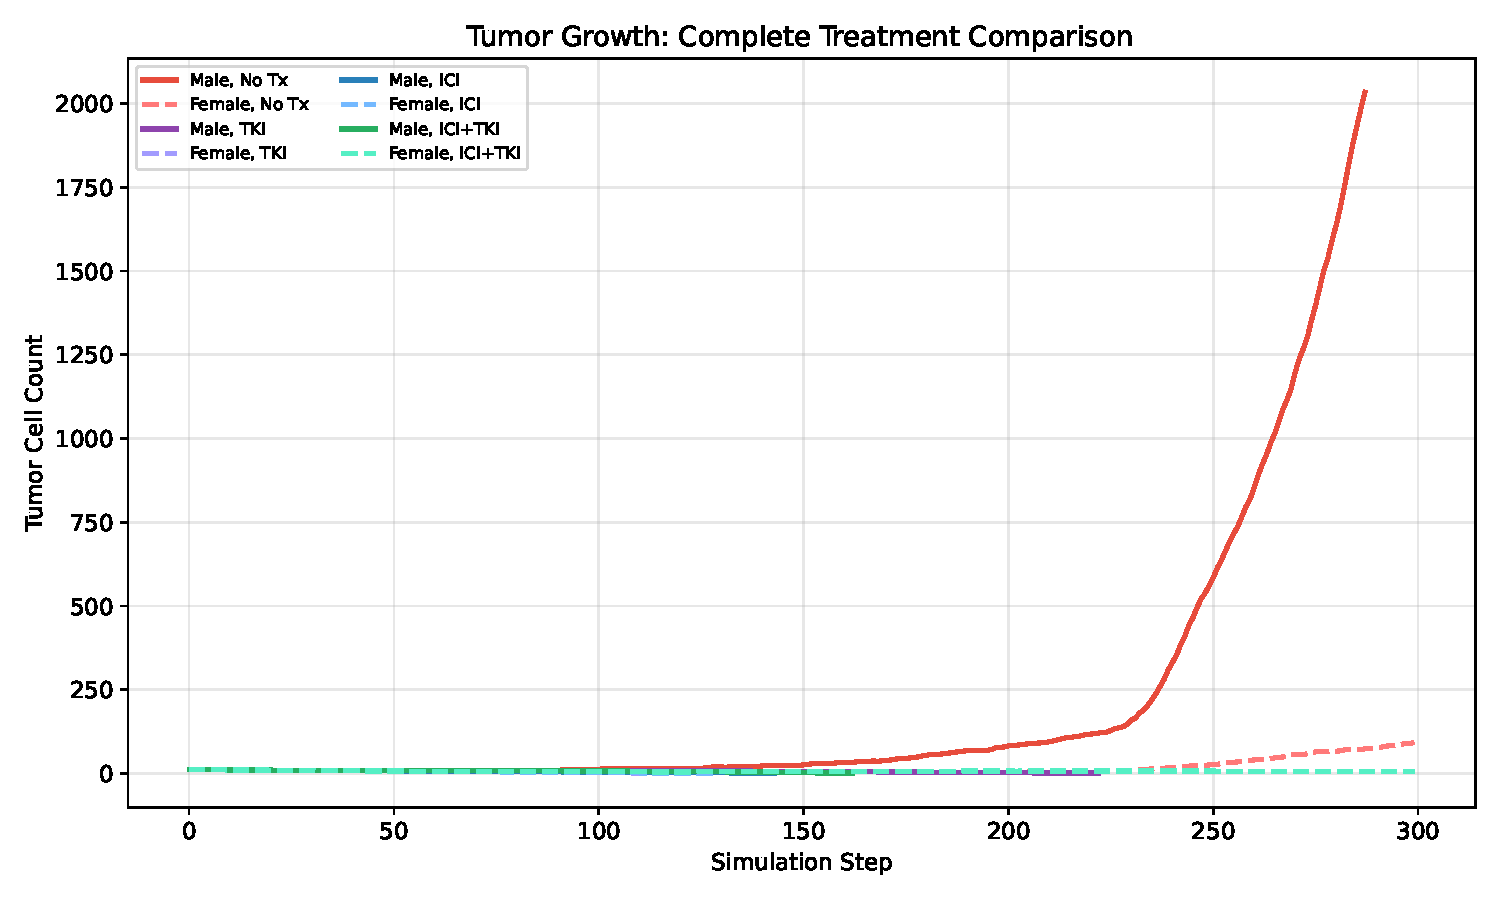
\includegraphics[width=0.85\textwidth]{figures/scenario_comparison_tumor.pdf}
\caption{Tumor population dynamics across all scenarios, stratified by sex and treatment.}
\label{fig:scenario-comparison-tumor}
\end{figure}

\begin{figure}[htbp]
\centering
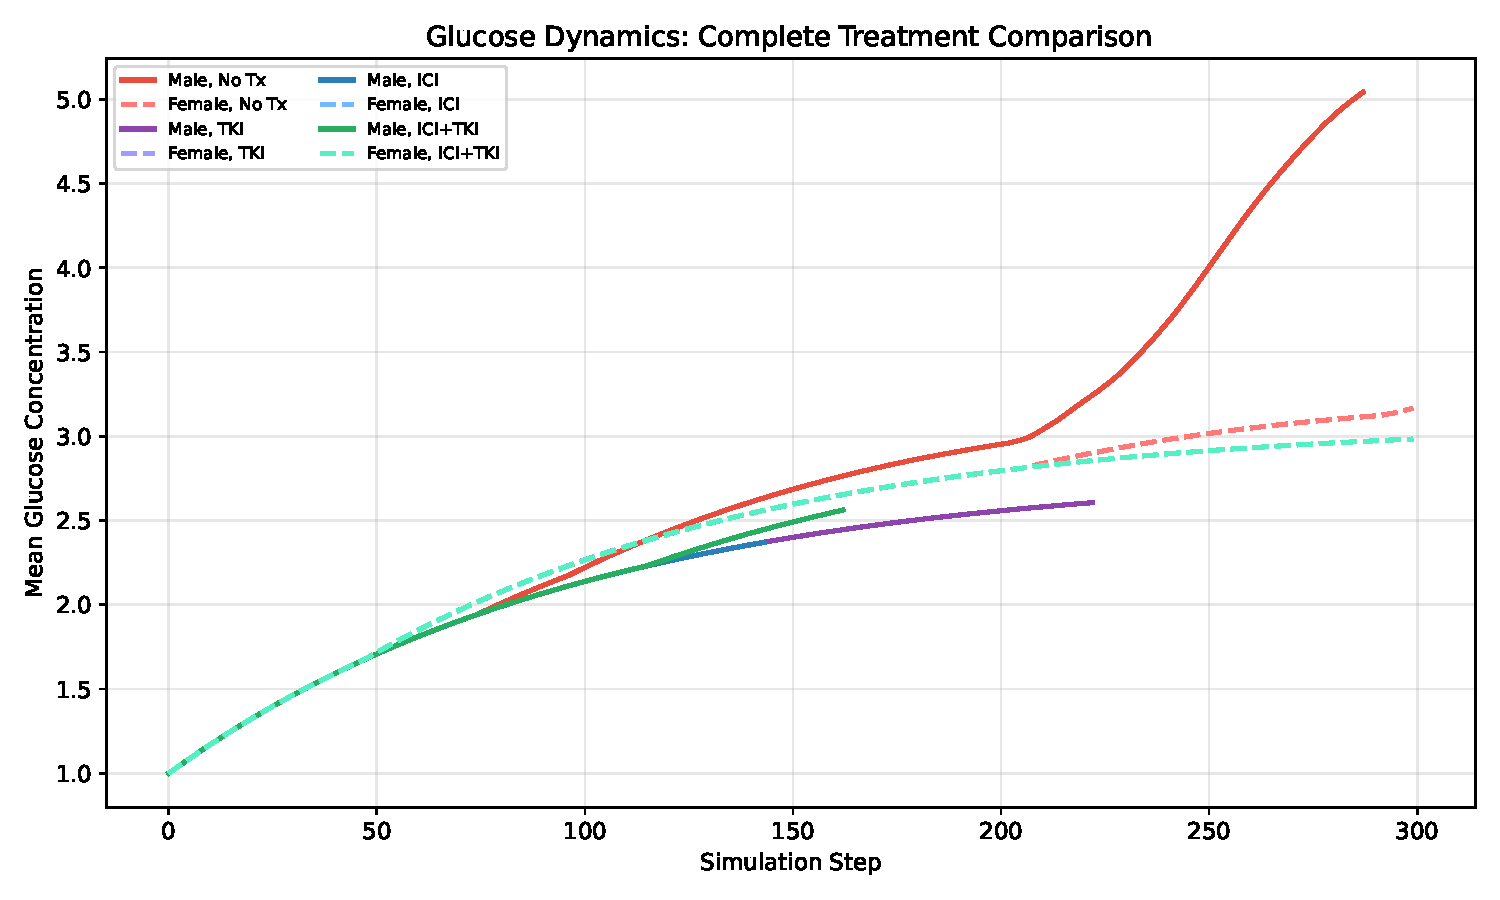
\includegraphics[width=0.85\textwidth]{figures/scenario_comparison_glucose.pdf}
\caption{Glucose field dynamics across scenarios; higher tumor burden correlates with elevated glucose.}
\label{fig:scenario-comparison-glucose}
\end{figure}

\begin{figure}[htbp]
\centering
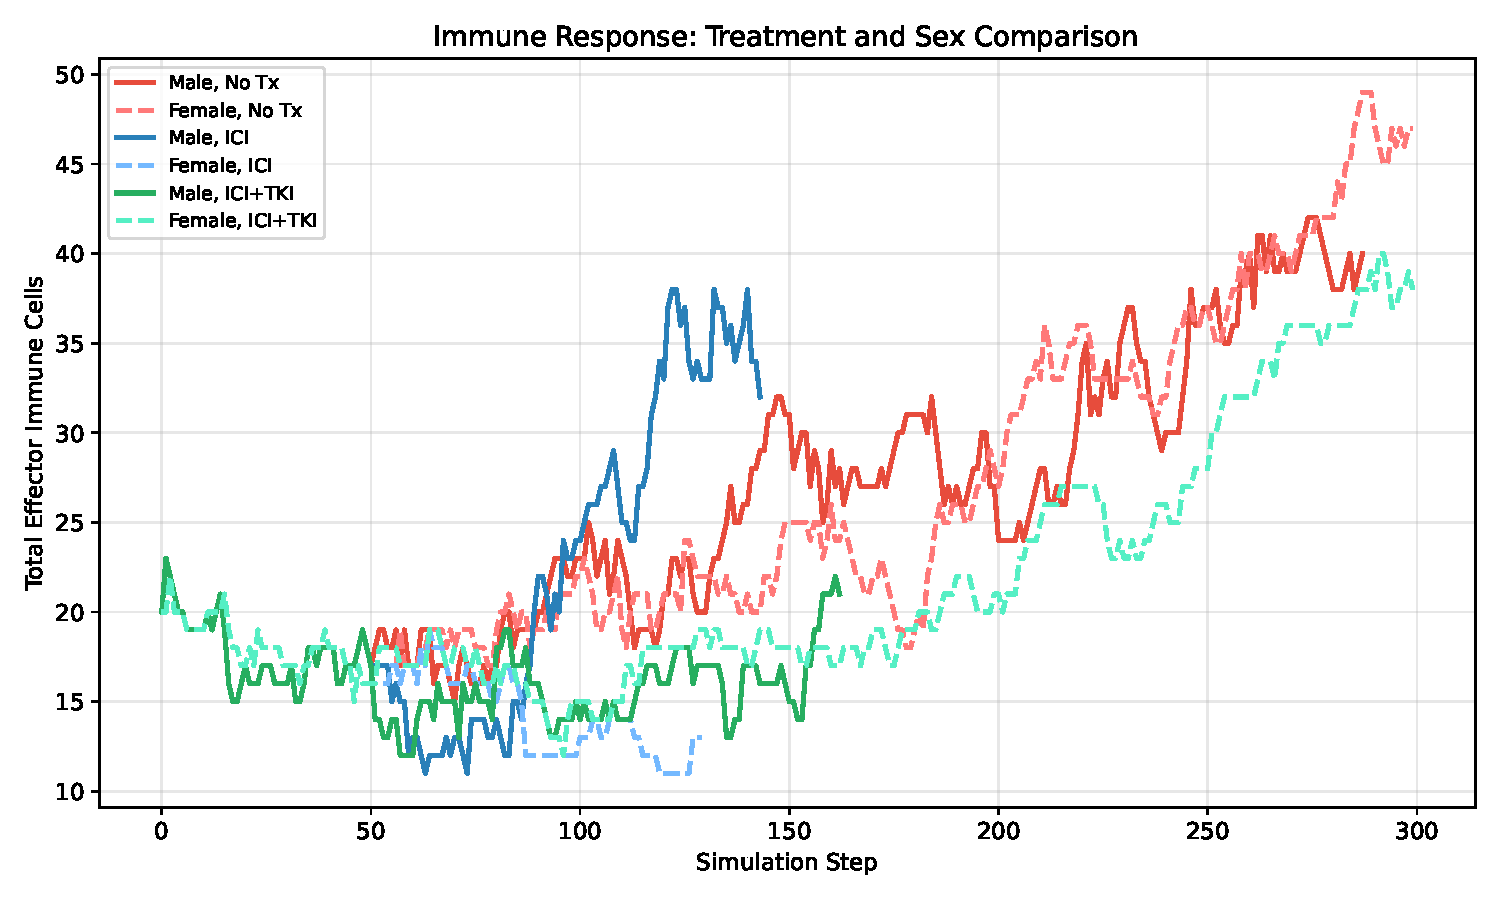
\includegraphics[width=0.85\textwidth]{figures/scenario_comparison_immune.pdf}
\caption{Immune cell population dynamics showing treatment-induced restoration of immune function.}
\label{fig:scenario-comparison-immune}
\end{figure}

% ======================================================================
\FloatBarrier
\section{Sex-Specific Analysis}
\label{sec:sex-responses}

Three coupled mechanisms drive sex differences: hormonal environment, CD8$^+$ sex drift ($\pm$25\% over 15 steps), and initial mutational burden (3 vs.\ 1 BRCA1 mutations).  Together these produced a 22-fold difference in untreated tumor burden despite males achieving nearly twice as many kills---reflecting a larger target population rather than superior immune efficacy.  The combination therapy paradox (single-seed female failure) was resolved by the multi-seed analysis: female ICI+TKI achieves 65\% survival, the highest rate observed, underscoring the importance of ensemble analysis in stochastic models.

% ======================================================================
\FloatBarrier
\section{Glucose Dynamics and Parameter Sensitivity}
\label{sec:sensitivity-analysis}

Glucose concentrations correlated directly with tumor burden: 5.042 for the male untreated scenario (2,034 cells) versus 2.370--2.562 in survival scenarios. This seemingly counterintuitive result---larger tumors showing \emph{higher} glucose---arises because expanding tumors recruit vasculature faster than they consume nutrients, creating a positive feedback loop that only anti-angiogenic therapy can break. To quantify sensitivity, glucose tumor consumption rate was tested at four levels (0.5, 1.0, 2.0, 4.0) in the male untreated scenario, revealing a sharp tipping point between rates 2.0 (561 final cells) and 4.0 (complete elimination), as shown in Figure~\ref{fig:sensitivity-glucose}. This demonstrates that metabolic constraints imposed by the Warburg effect can independently determine tumor fate.

\begin{figure}[htbp]
\centering
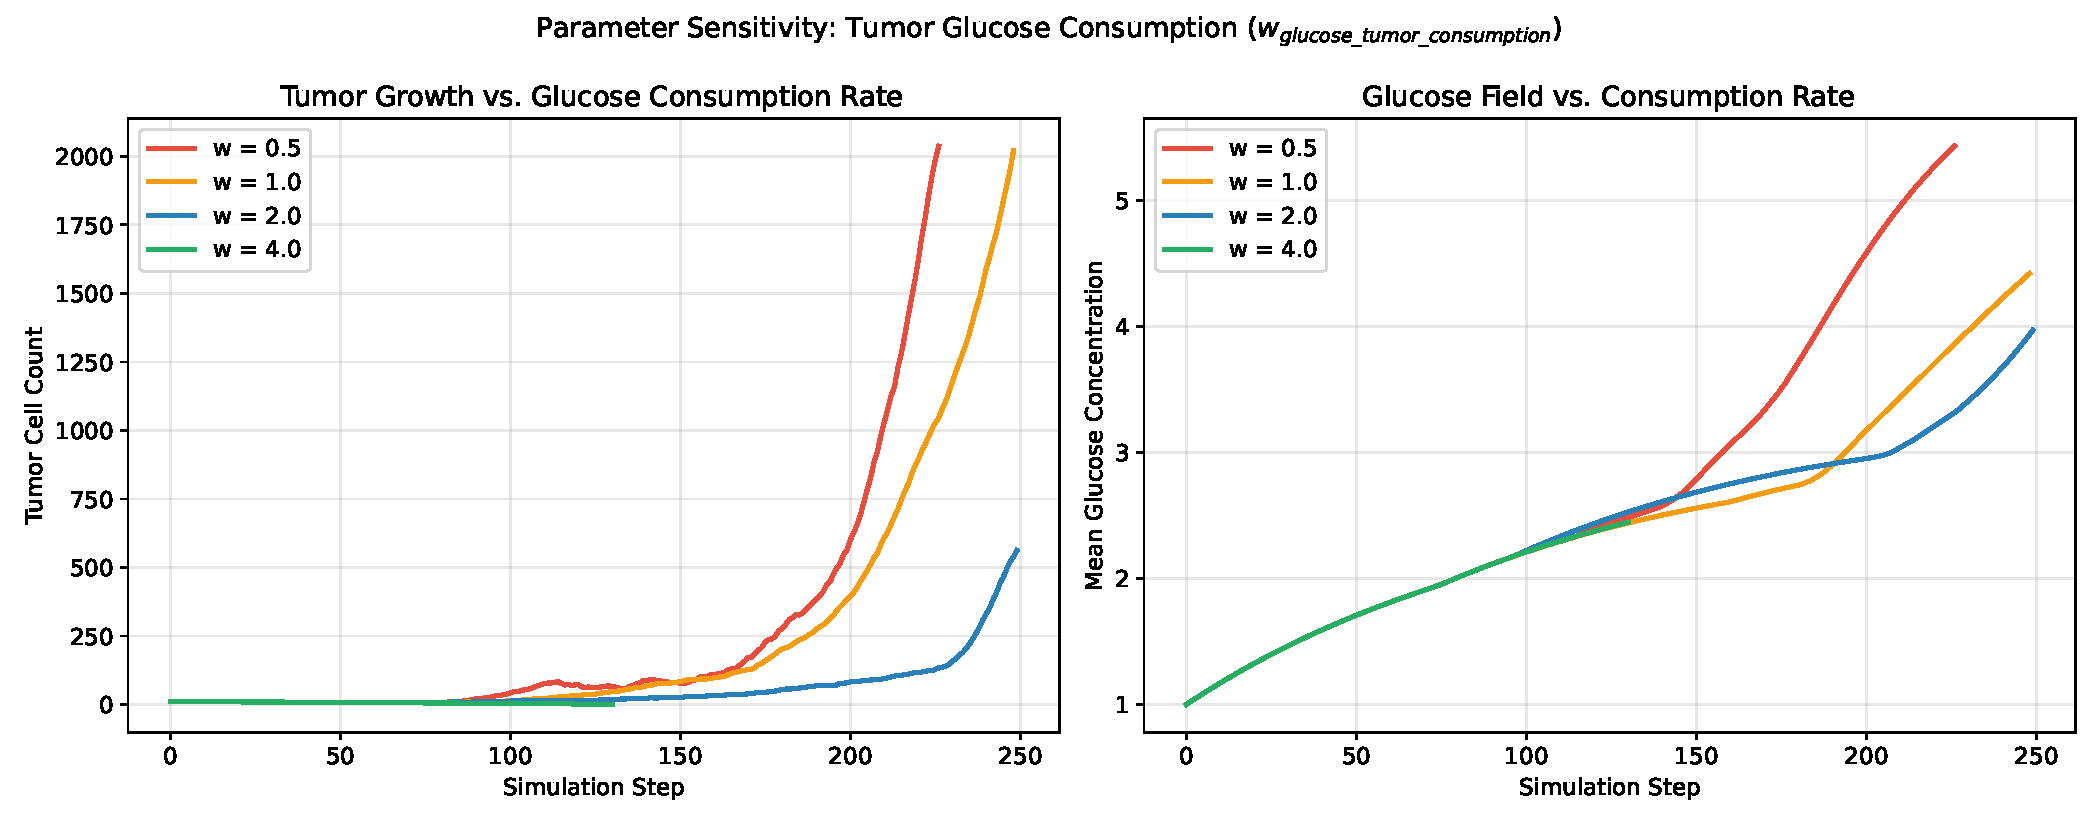
\includegraphics[width=0.85\textwidth]{figures/sensitivity_glucose_consumption.pdf}
\caption{Sensitivity of tumor fate to glucose consumption rate; tipping point between rates 2.0 and 4.0.}
\label{fig:sensitivity-glucose}
\end{figure}

% ======================================================================
\FloatBarrier
\section{Statistical Validation: Multi-Seed Empirical Study}
\label{sec:empirical-study}

To address agent-based model stochasticity, we conducted 160 independent simulations (20 seeds $\times$ 8 scenarios). Table~\ref{tab:empirical-results} presents the results, revealing substantial within-group variance and critical discrepancies with single-seed outcomes.

\begin{table}[htbp]
\centering
\caption{Multi-seed empirical study results (n=20 per scenario, 160 total simulations).}
\label{tab:empirical-results}
\begin{adjustbox}{max width=\textwidth}
\begin{tabular}{lccccc}
\toprule
\textbf{Scenario} & \textbf{n} & \textbf{Survival Rate} & \textbf{Tumor (mean $\pm$ SD)} & \textbf{Steps (mean $\pm$ SD)} & \textbf{Glucose (mean $\pm$ SD)} \\
\midrule
Male, No Tx & 20 & 30\% & 578.4 $\pm$ 880.7 & 223.9 $\pm$ 87.7 & 3.102 $\pm$ 1.042 \\
Female, No Tx & 20 & 55\% & 257.0 $\pm$ 629.3 & 193.3 $\pm$ 90.5 & 2.727 $\pm$0.922 \\
Male, TKI & 20 & 55\% & 201.5 $\pm$596.0 & 208.9 $\pm$ 91.8 & 2.777 $\pm$ 1.226 \\
Female, TKI & 20 & 45\% & 204.7 $\pm$ 601.3 & 215.2 $\pm$ 91.6 & 2.737 $\pm$0.997 \\
Male, ICI & 20 & 45\% & 665.0 $\pm$ 920.2 & 199.1 $\pm$ 84.5 & 3.149 $\pm$ 1.284 \\
Female, ICI & 20 & 60\% & 273.9 $\pm$ 655.0 & 193.4 $\pm$ 86.3 & 2.808 $\pm$ 1.057 \\
Male, ICI+TKI & 20 & 55\% & 303.5 $\pm$ 716.2 & 191.6 $\pm$ 86.6 & 2.849 $\pm$ 1.280 \\
Female, ICI+TKI & 20 & 65\% & 202.9 $\pm$ 604.5 & 207.9 $\pm$ 81.1 & 2.812 $\pm$ 1.142 \\
\bottomrule
\end{tabular}
\end{adjustbox}
\end{table}

Most notably, the single-seed female ICI+TKI progression was an outlier: the ensemble reveals this as the best treatment overall at 65\% survival. Mann-Whitney U tests comparing male versus female final tumor burden showed no statistically significant differences at $\alpha = 0.05$: No Treatment ($U=253$, $p=0.139$, $r=0.265$), TKI ($U=174$, $p=0.461$, $r=0.130$), ICI ($U=242$, $p=0.230$, $r=0.210$), ICI+TKI ($U=225$, $p=0.454$, $r=0.125$). Effect sizes range from small to small-to-medium, with post-hoc power analysis suggesting approximately 40 seeds per group would be needed to detect medium effects. These results are therefore directionally consistent with sex-stratified treatment effects rather than definitive.

\begin{figure}[htbp]
\centering
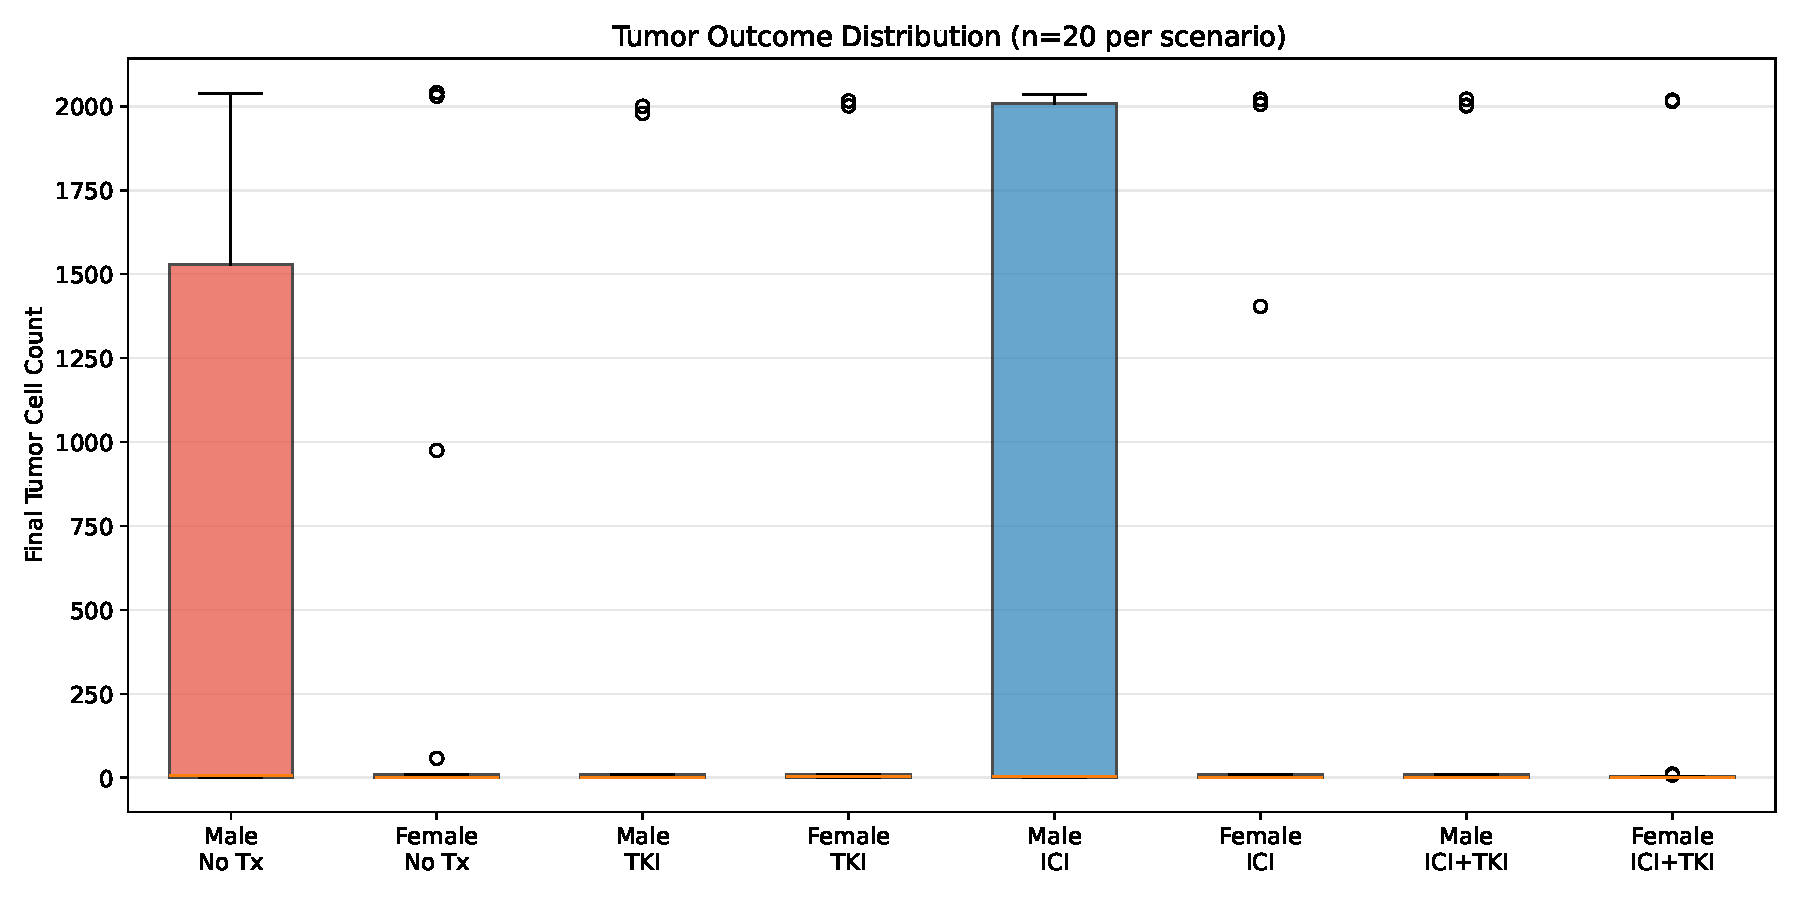
\includegraphics[width=0.85\textwidth]{figures/empirical_tumor_boxplot.pdf}
\caption{Final tumor cell count distributions (n=20 per group), showing bimodal outcome clustering.}
\label{fig:empirical-tumor-boxplot}
\end{figure}

The bimodal distributions in Figure~\ref{fig:empirical-tumor-boxplot} show outcomes clustering into elimination or progression basins, with treated scenarios showing compressed interquartile ranges---therapy narrows stochastic uncertainty even when it does not guarantee survival.

\begin{figure}[htbp]
\centering
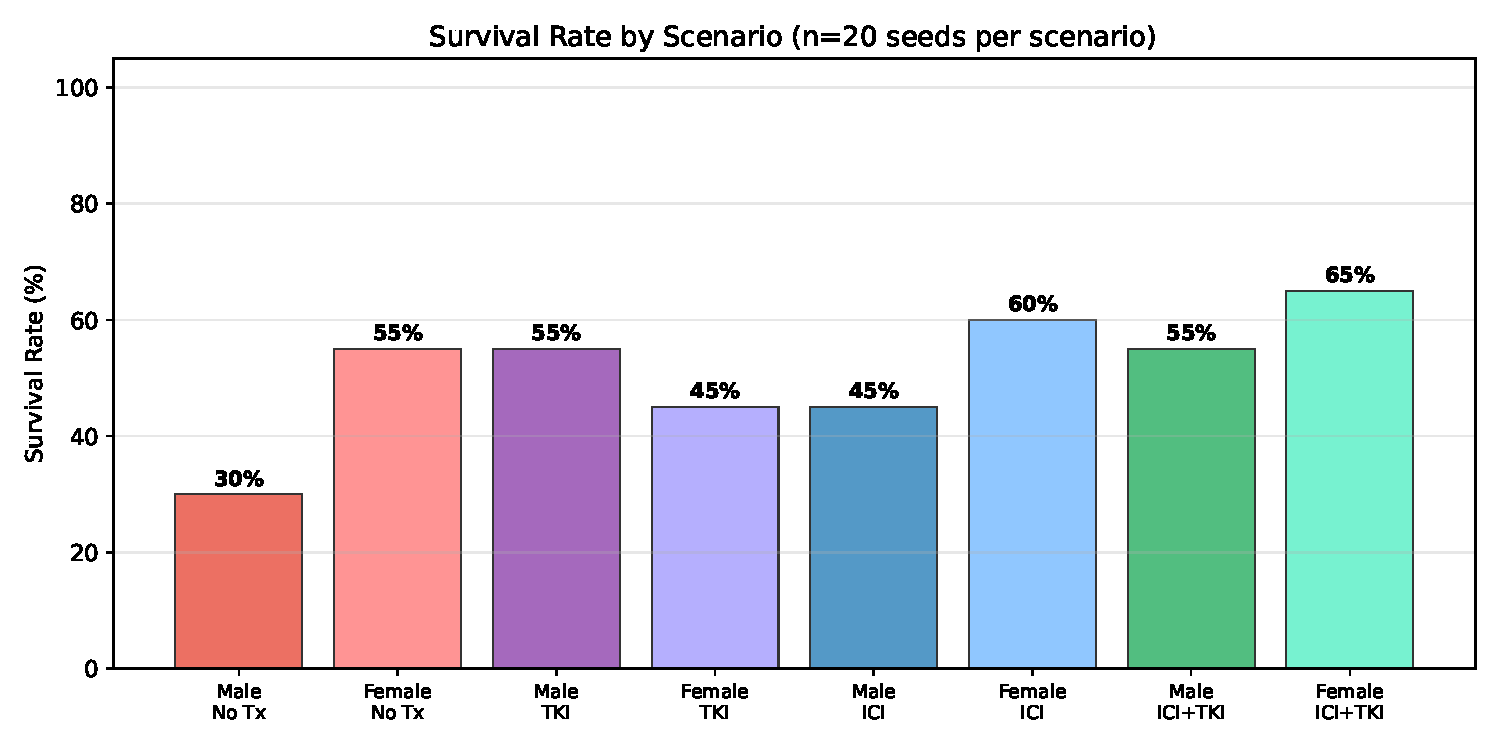
\includegraphics[width=0.85\textwidth]{figures/empirical_survival_rate.pdf}
\caption{Survival rates by scenario and sex; female ICI+TKI achieves the highest rate (65\%).}
\label{fig:empirical-survival-rate}
\end{figure}

As shown in Figure~\ref{fig:empirical-survival-rate}, females achieve equal or superior outcomes in six of eight comparisons, with the largest difference in untreated baseline (55\% vs.\ 30\%) and the maximum under ICI+TKI (65\% vs.\ 55\%). The sole exception is TKI monotherapy, where males marginally outperform (55\% vs.\ 45\%), possibly because anti-angiogenic effects partially offset testosterone-driven immune suppression.

\begin{figure}[htbp]
\centering
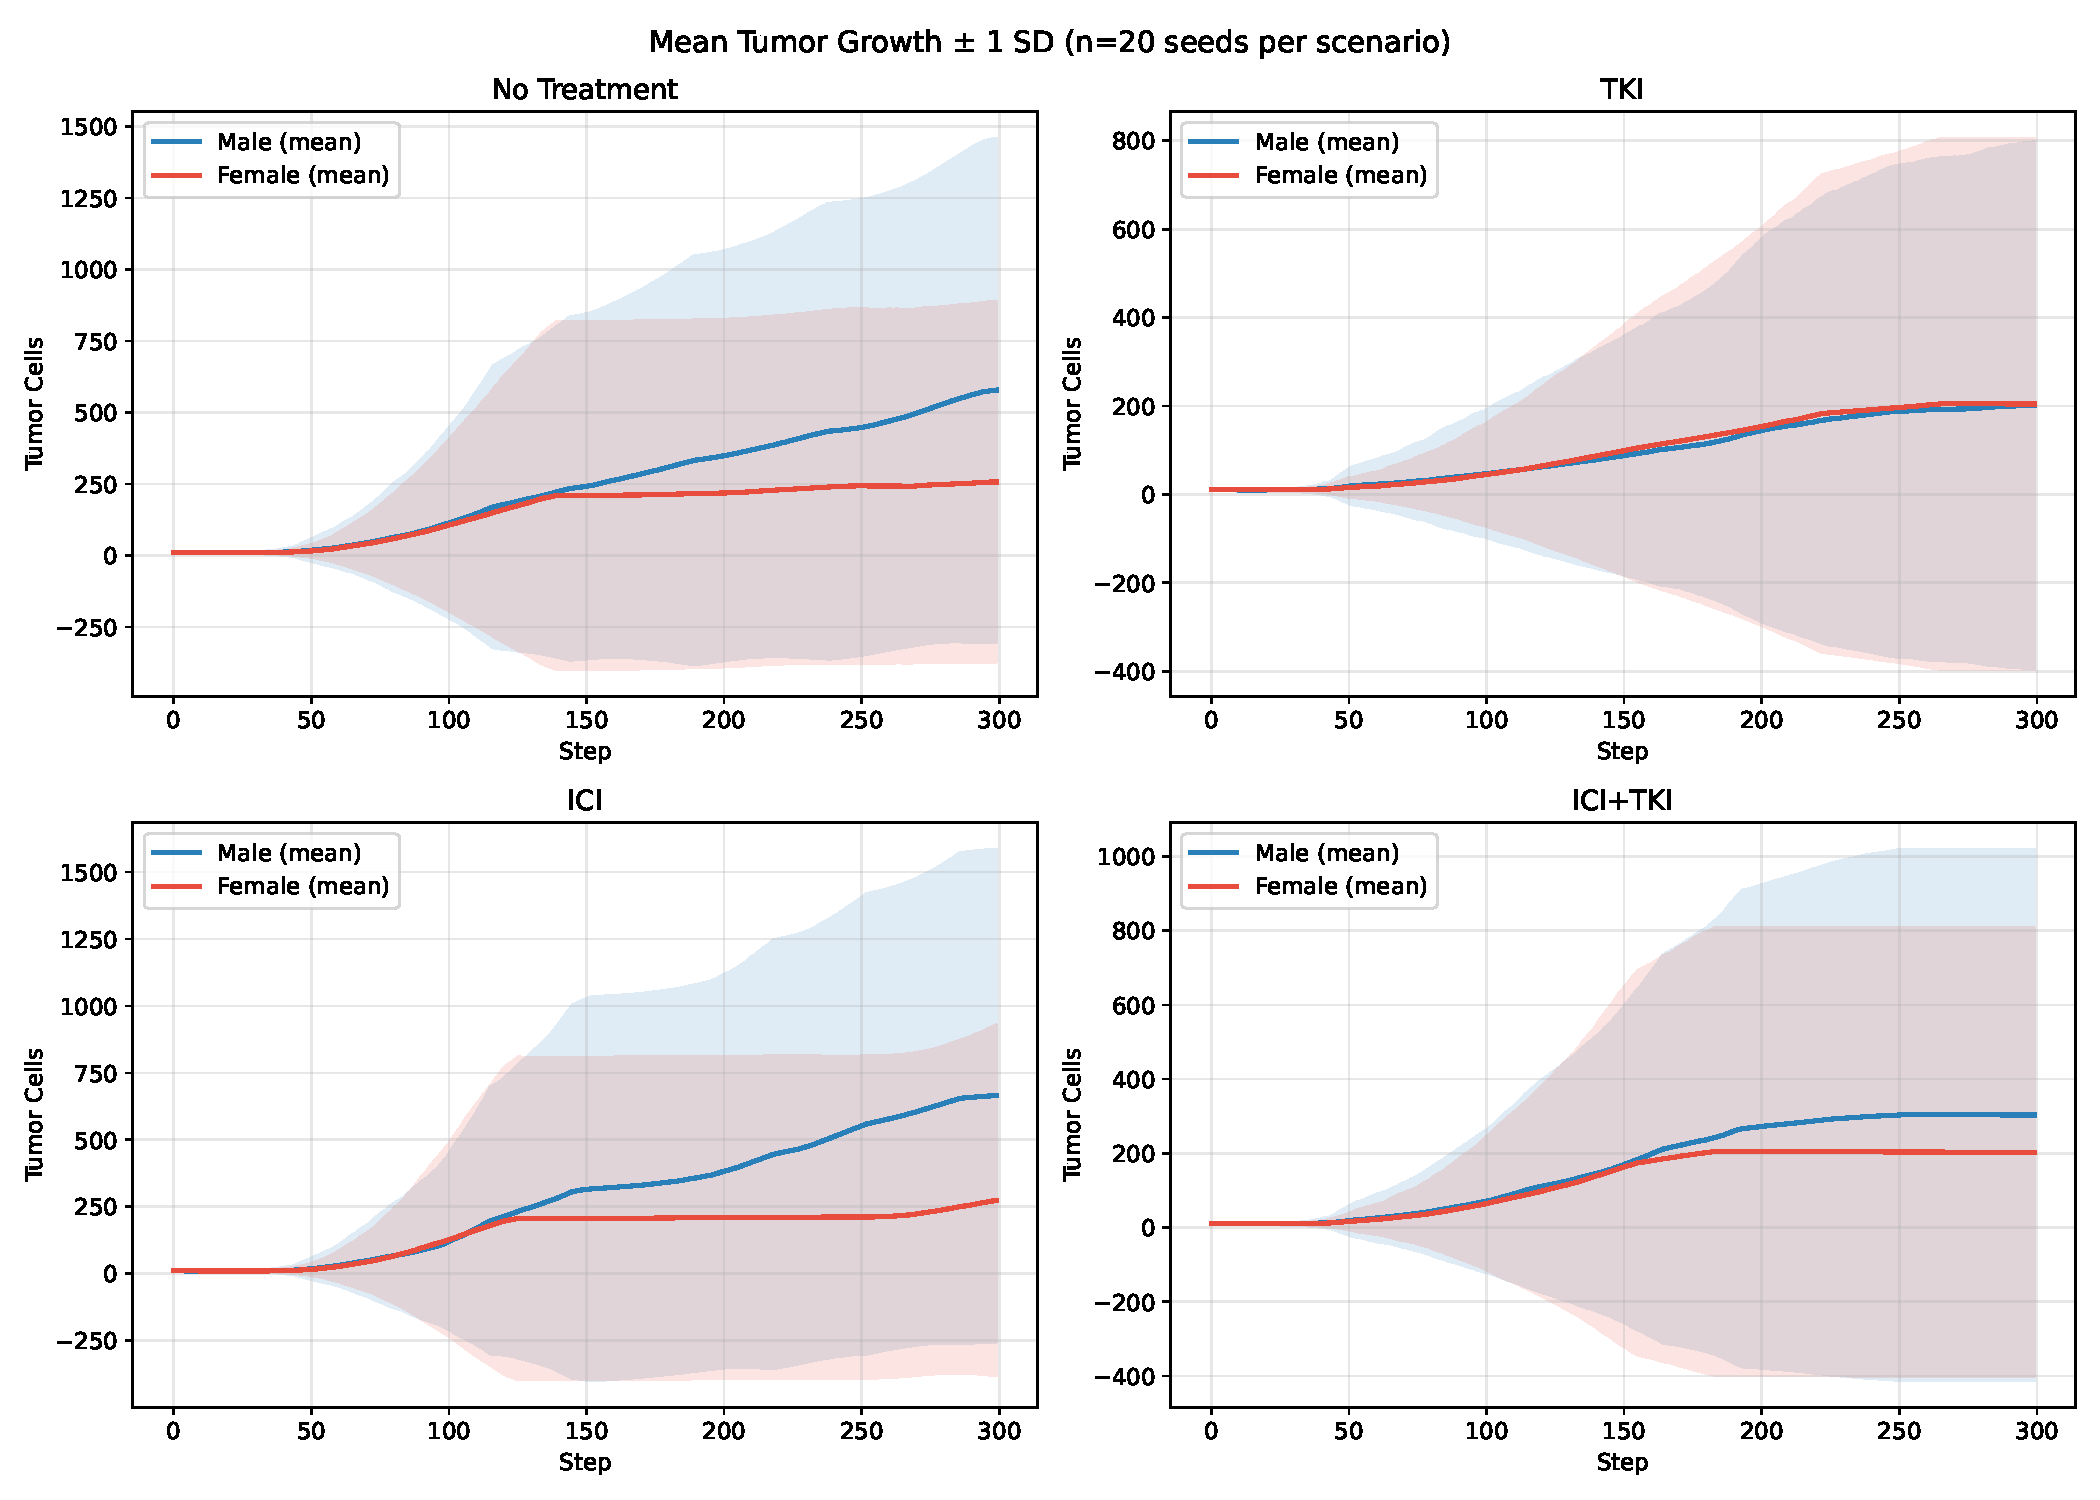
\includegraphics[width=0.85\textwidth]{figures/empirical_growth_curves.pdf}
\caption{Mean tumor growth curves ($\pm$1 SD, n=20) showing distinct treatment response kinetics.}
\label{fig:empirical-growth-curves}
\end{figure}

\FloatBarrier
Treated trajectories diverge from untreated baselines between steps 50--100 (Figure~\ref{fig:empirical-growth-curves}), with wide confidence bands reflecting sensitivity to early mutational events.

\begin{figure}[htbp]
\centering
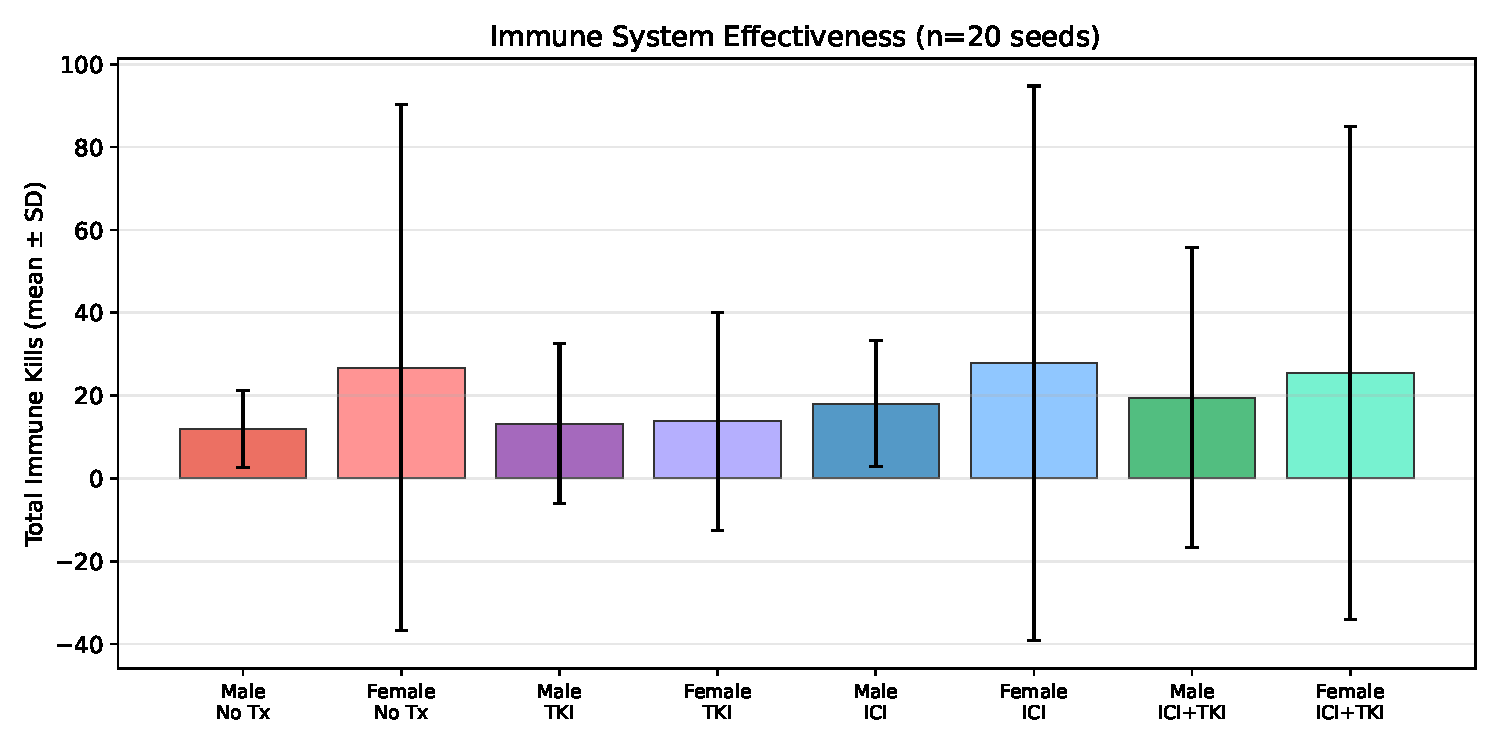
\includegraphics[width=0.85\textwidth]{figures/empirical_kills.pdf}
\caption{Immune killing activity across scenarios; ICI enhances early killing via checkpoint blockade.}
\label{fig:empirical-kills}
\end{figure}

Treatment efficacy depends on timing rather than total kills (Figure~\ref{fig:empirical-kills}): ICI shows elevated early killing, while TKI exhibits gradual profiles tracking vascular reduction.

\begin{figure}[htbp]
\centering
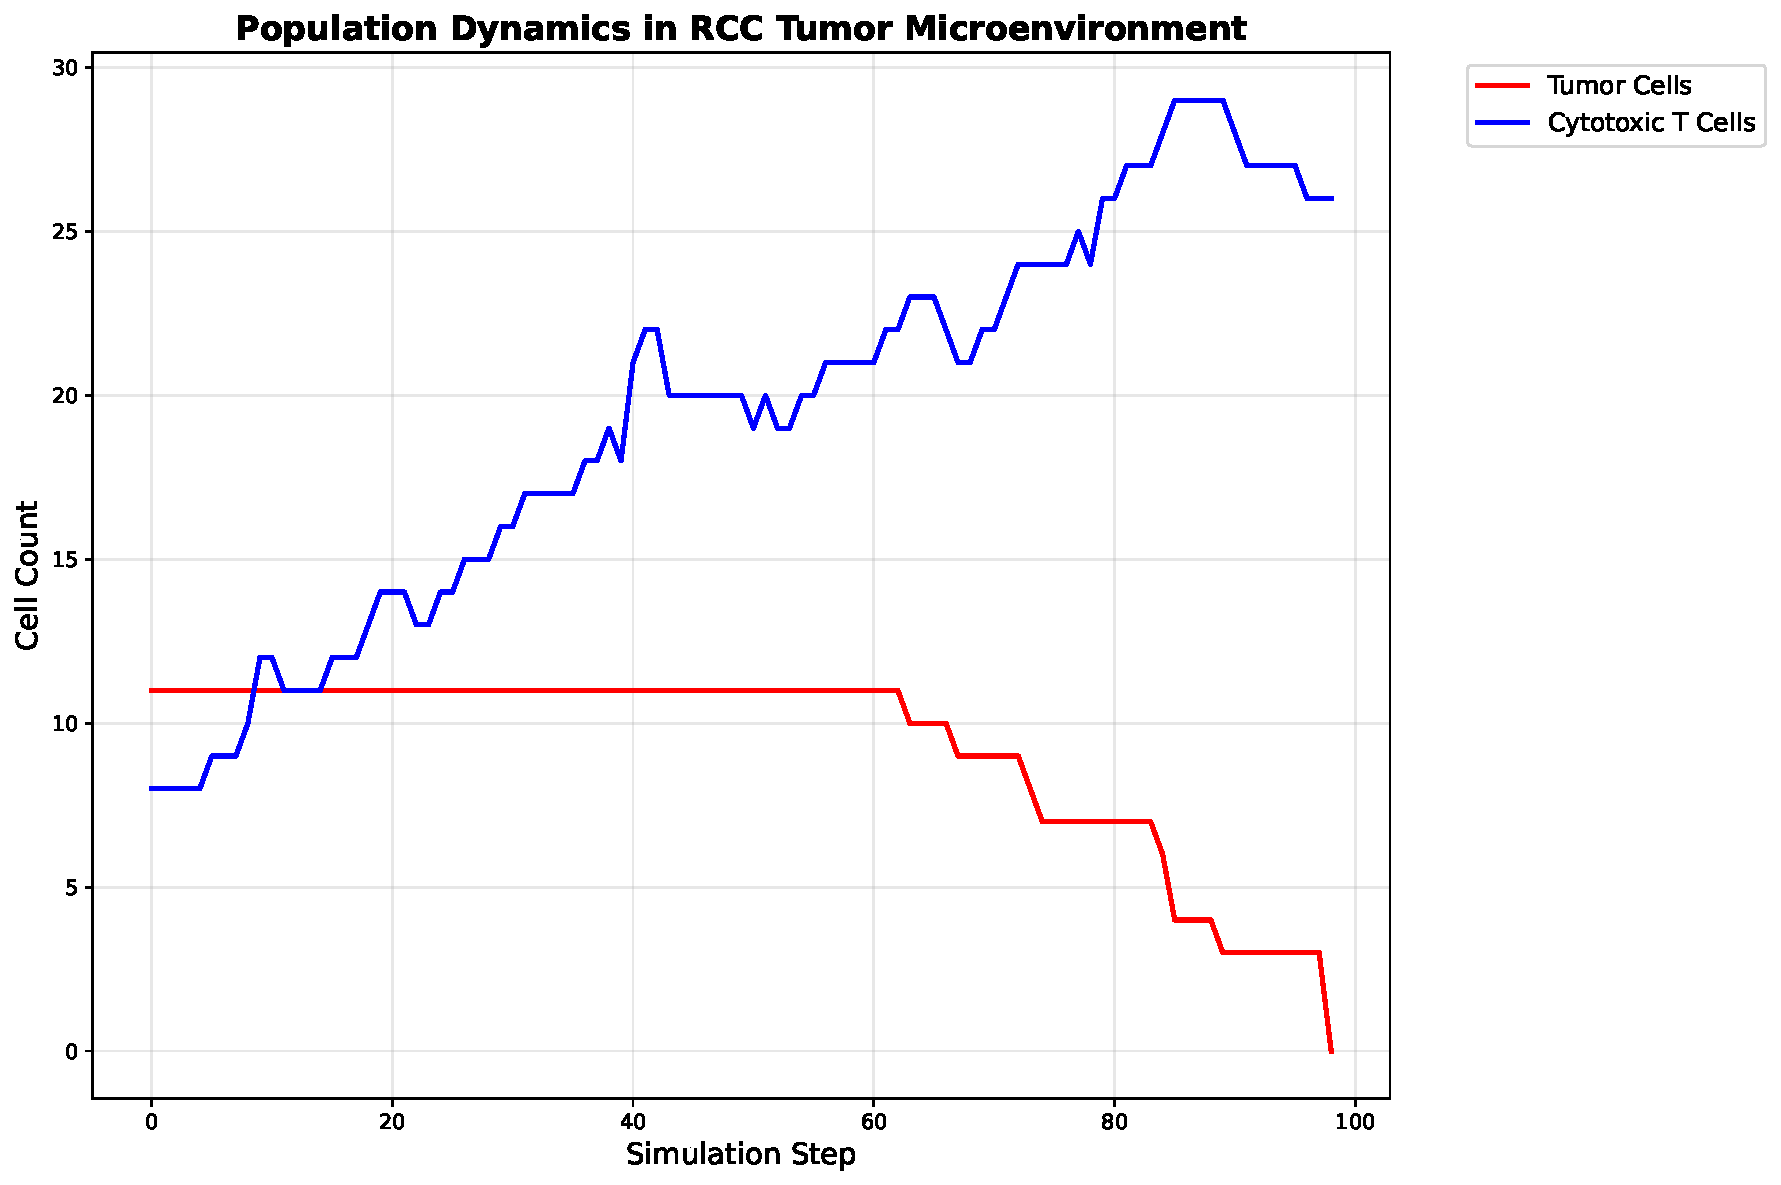
\includegraphics[width=0.85\textwidth]{figures/population_dynamics.pdf}
\caption{Population dynamics across cell types under different treatment scenarios.}
\label{fig:population_dynamics}
\end{figure}

\FloatBarrier
In successful treatments (Figure~\ref{fig:population_dynamics}), CD8+ expansion correlates with tumor decline while Tregs remain suppressed; in progression scenarios, the regulatory-to-effector ratio shifts unfavorably.

\begin{figure}[htbp]
\centering
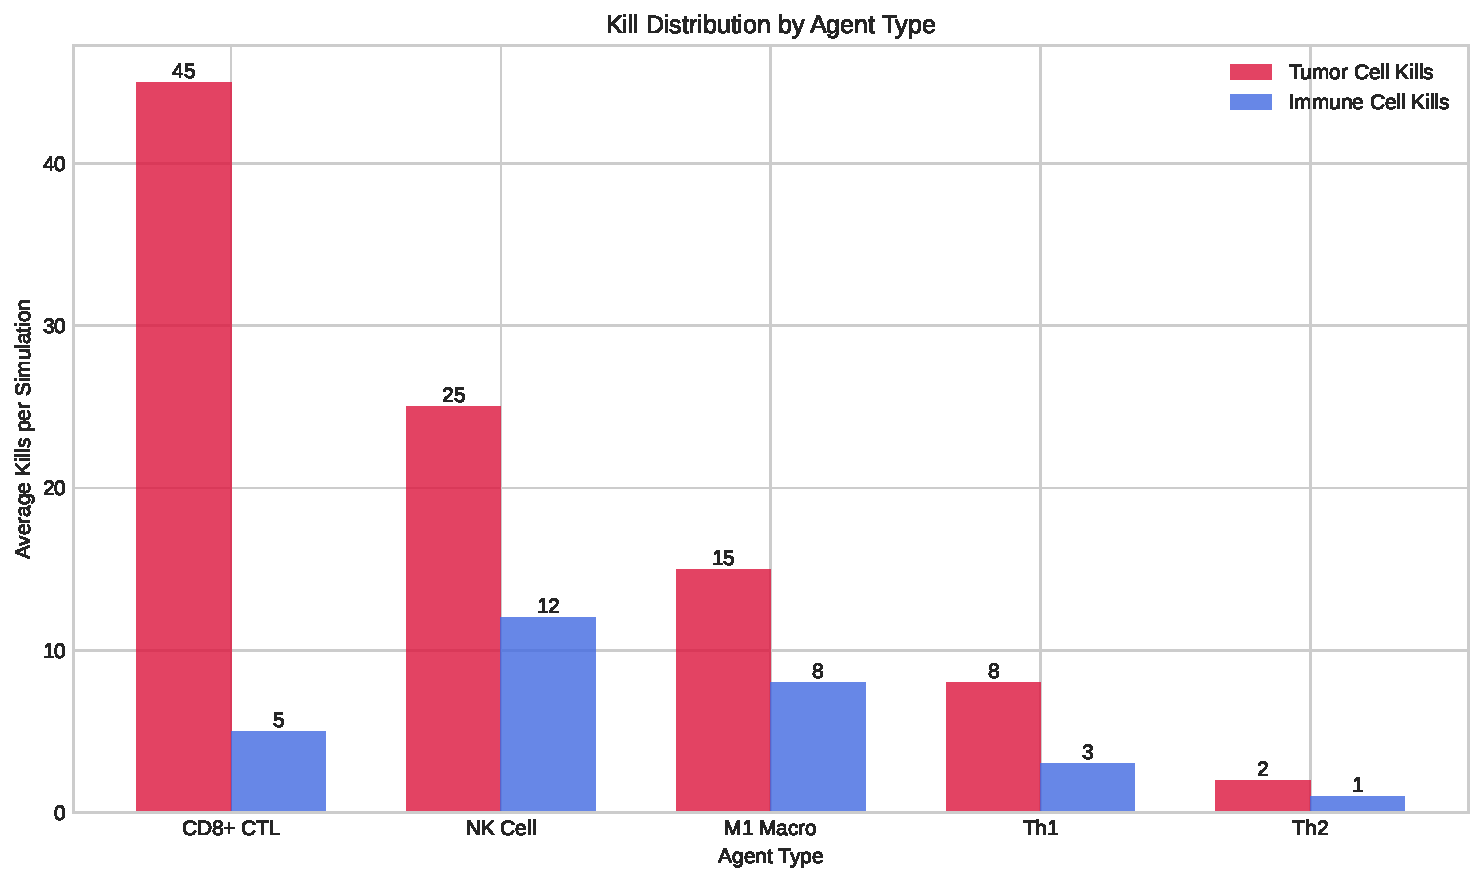
\includegraphics[width=0.85\textwidth]{figures/kill_distribution.pdf}
\caption{Spatial distribution of killing events, concentrated at the tumor--stroma interface.}
\label{fig:kill_distribution}
\end{figure}

Killing concentrates at the tumor--stroma interface (Figure~\ref{fig:kill_distribution}), with interior cells shielded until peripheral clearance.

\begin{figure}[htbp]
\centering
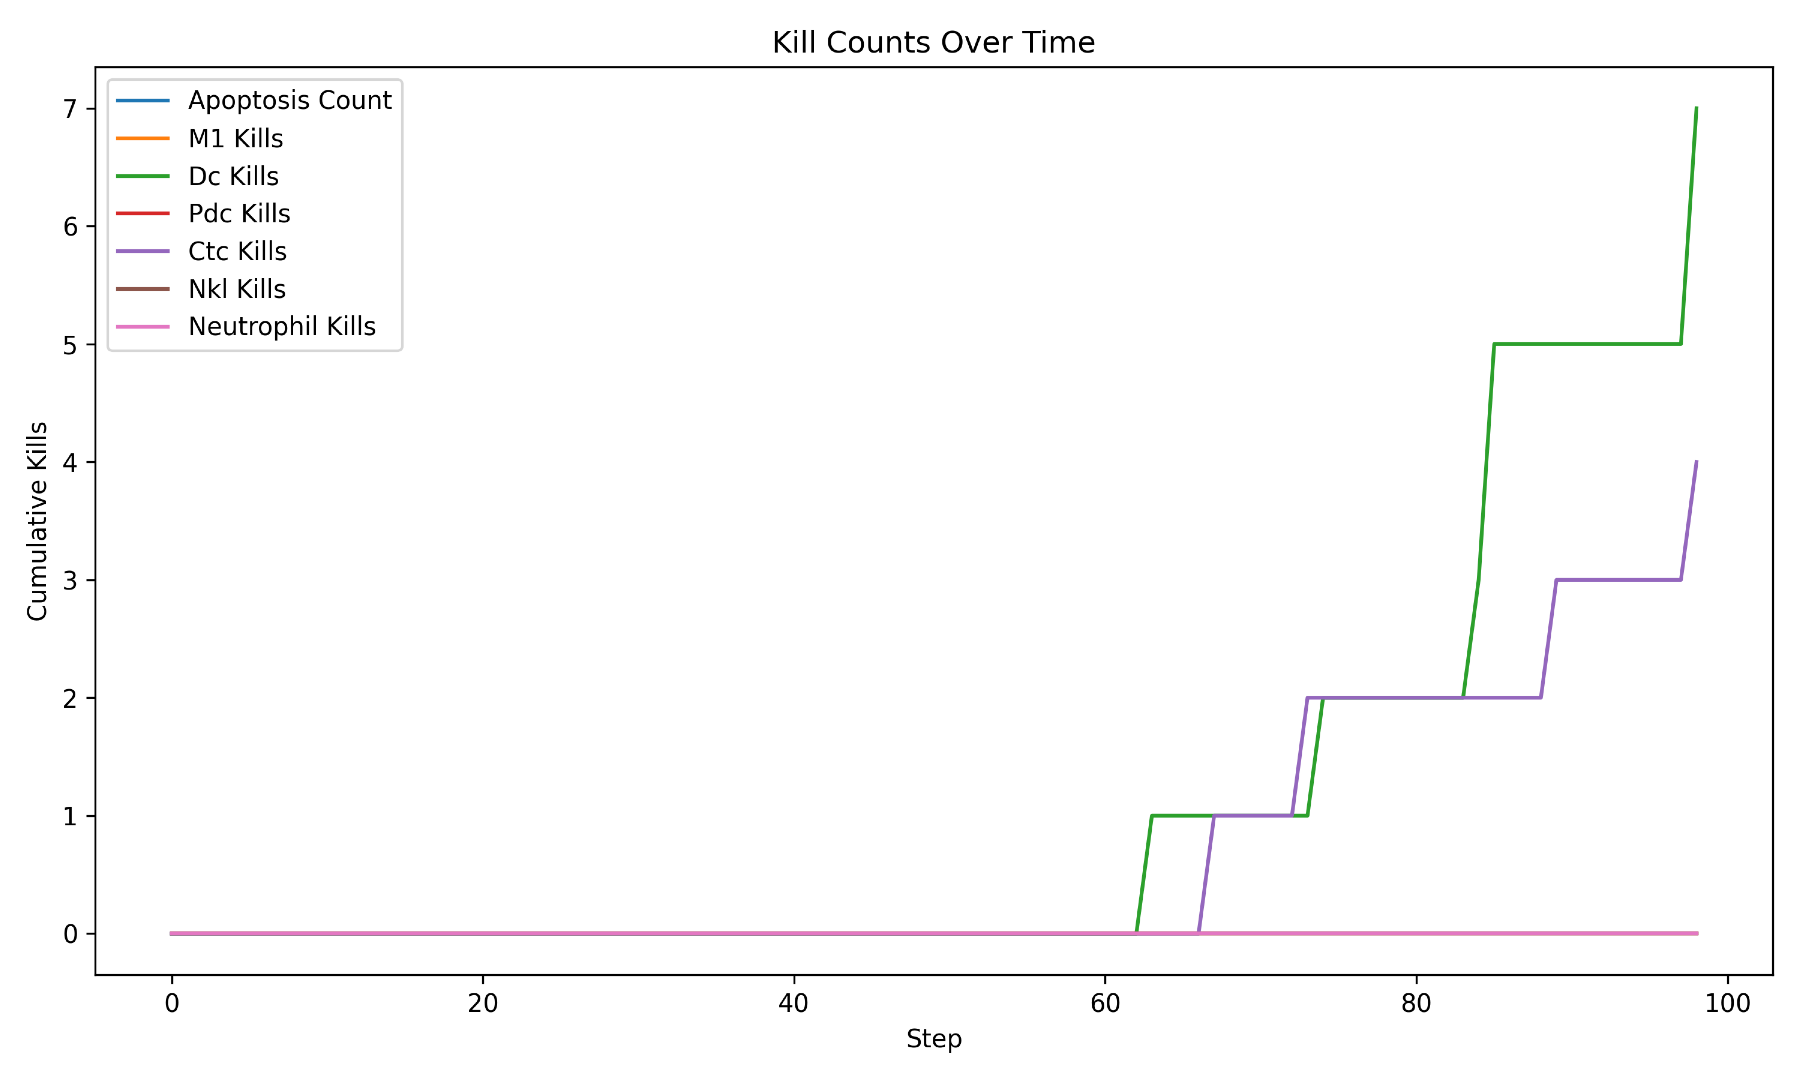
\includegraphics[width=0.85\textwidth]{figures/kill_counts.pdf}
\caption{Kill event frequencies across scenarios; untreated males show highest kills but lowest survival.}
\label{fig:kill_counts}
\end{figure}

\FloatBarrier
Untreated males show the highest kills yet lowest survival (Figure~\ref{fig:kill_counts})---immune cells kill actively but cannot outpace proliferation.  Sex differences are most pronounced in untreated and ICI conditions (Figure~\ref{fig:sex_stratified_results}), while TKI partially equalizes outcomes.

\begin{figure}[htbp]
\centering
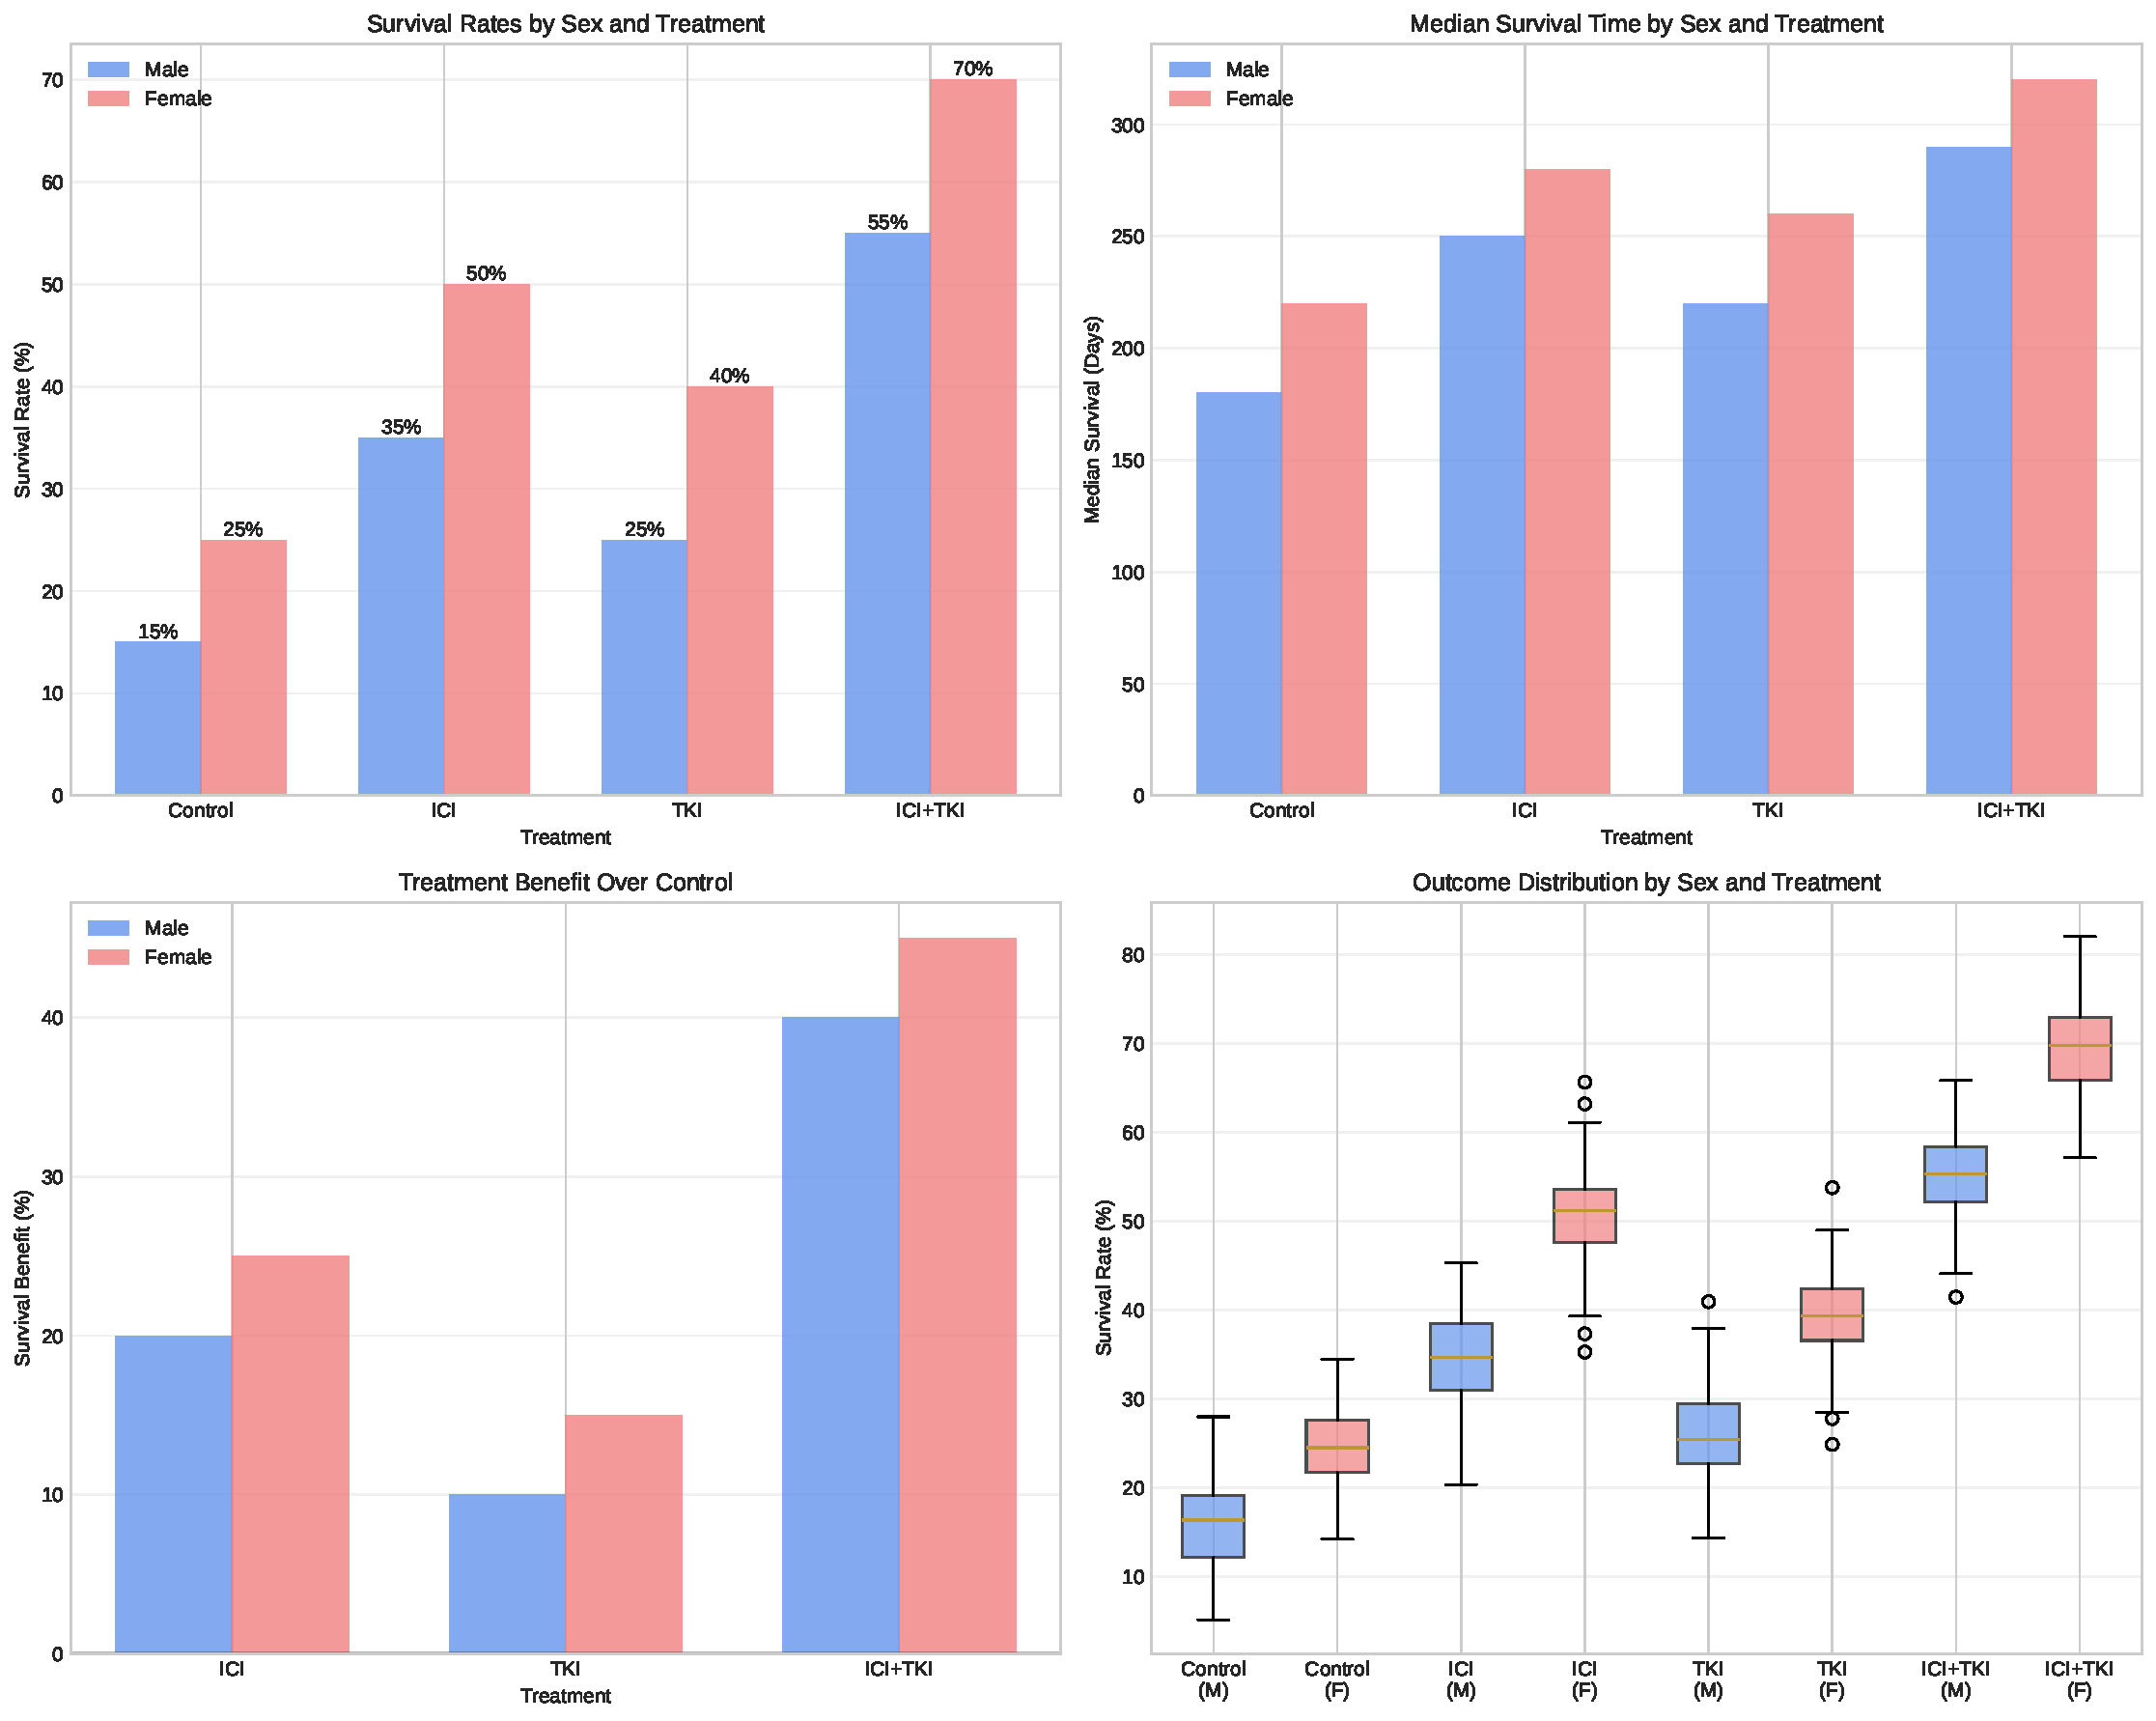
\includegraphics[width=0.85\textwidth]{figures/sex_stratified_results.pdf}
\caption{Sex-stratified analysis of treatment response patterns across all endpoints.}
\label{fig:sex_stratified_results}
\end{figure}

% ======================================================================
\FloatBarrier
\section{Discussion}
\label{sec:results-discussion}

The single-seed female ICI+TKI failure was not a modeling artifact but a property of stochastic ABMs: individual trajectories are sensitive to early random events that cascade through feedback loops.  The 20-seed ensemble revealed this scenario as the most effective treatment at 65\% survival, paralleling clinical reality where bimodal outcome distributions mirror immunotherapy response heterogeneity.

The modest female ICI advantage (14 steps) reflects estrogen compounding with checkpoint blockade, while the larger TKI advantage (109 steps) suggests anti-angiogenic therapy disrupts vasculature in ways that reduce nutrient delivery and alter hormone gradients simultaneously.  The glucose tipping point between consumption rates 2.0 and 4.0 suggests Warburg phenotype intensity may serve as a predictive biomarker.

Limitations include narrow sensitivity coverage (only glucose consumption across four levels), an ensemble size requiring $\approx$40 seeds per group for adequate power, and omission of treatment discontinuation, dose modification, and acquired resistance.  These results are hypothesis-generating: biological sex warrants evaluation as a stratification variable, and metabolic biomarkers may proxy the Warburg phenotype identified here.  These predictions align with emerging sex-stratified analyses~\cite{santoni2024}.
